% !Rnw weave = knitr  
\documentclass[12pt, a4paper]{article}\usepackage[]{graphicx}\usepackage[]{xcolor}
% maxwidth is the original width if it is less than linewidth
% otherwise use linewidth (to make sure the graphics do not exceed the margin)
\makeatletter
\def\maxwidth{ %
  \ifdim\Gin@nat@width>\linewidth
    \linewidth
  \else
    \Gin@nat@width
  \fi
}
\makeatother

\definecolor{fgcolor}{rgb}{0.345, 0.345, 0.345}
\newcommand{\hlnum}[1]{\textcolor[rgb]{0.686,0.059,0.569}{#1}}%
\newcommand{\hlstr}[1]{\textcolor[rgb]{0.192,0.494,0.8}{#1}}%
\newcommand{\hlcom}[1]{\textcolor[rgb]{0.678,0.584,0.686}{\textit{#1}}}%
\newcommand{\hlopt}[1]{\textcolor[rgb]{0,0,0}{#1}}%
\newcommand{\hlstd}[1]{\textcolor[rgb]{0.345,0.345,0.345}{#1}}%
\newcommand{\hlkwa}[1]{\textcolor[rgb]{0.161,0.373,0.58}{\textbf{#1}}}%
\newcommand{\hlkwb}[1]{\textcolor[rgb]{0.69,0.353,0.396}{#1}}%
\newcommand{\hlkwc}[1]{\textcolor[rgb]{0.333,0.667,0.333}{#1}}%
\newcommand{\hlkwd}[1]{\textcolor[rgb]{0.737,0.353,0.396}{\textbf{#1}}}%
\let\hlipl\hlkwb

\usepackage{framed}
\makeatletter
\newenvironment{kframe}{%
 \def\at@end@of@kframe{}%
 \ifinner\ifhmode%
  \def\at@end@of@kframe{\end{minipage}}%
  \begin{minipage}{\columnwidth}%
 \fi\fi%
 \def\FrameCommand##1{\hskip\@totalleftmargin \hskip-\fboxsep
 \colorbox{shadecolor}{##1}\hskip-\fboxsep
     % There is no \\@totalrightmargin, so:
     \hskip-\linewidth \hskip-\@totalleftmargin \hskip\columnwidth}%
 \MakeFramed {\advance\hsize-\width
   \@totalleftmargin\z@ \linewidth\hsize
   \@setminipage}}%
 {\par\unskip\endMakeFramed%
 \at@end@of@kframe}
\makeatother

\definecolor{shadecolor}{rgb}{.97, .97, .97}
\definecolor{messagecolor}{rgb}{0, 0, 0}
\definecolor{warningcolor}{rgb}{1, 0, 1}
\definecolor{errorcolor}{rgb}{1, 0, 0}
\newenvironment{knitrout}{}{} % an empty environment to be redefined in TeX

\usepackage{alltt}
\usepackage[T1]{fontenc}
\usepackage{graphicx}
\usepackage{float}
\usepackage[colorlinks=true, linkcolor=blue]{hyperref}
\usepackage{amsmath, amsthm, amssymb, amscd}
\usepackage{enumerate}
\usepackage{polski}
%%%%%%%%%%%%%%%%%%%%%%%%%%%%%%%%%%%%%%%%%%%%%%%%%%%%%%%%%%%%%%%%%%%%%%%%%%%%%%%%
%%%%%%%%%%%%%%%%%%%%%%%%%%%%%%%%%%%%%%%%%%%%%%%%%%%%%%%%%%%%%%%%%%%%%%%%%%%%%%%%
\usepackage[top=2.5cm, bottom=2.5cm, left=2cm, right=2cm]{geometry}
\makeatletter
\newcommand\numerraportu[1]{\renewcommand\@title{Raport #1}}
\renewcommand{\maketitle}{
    \begin{center}
        \vspace{5pt}
        \textbf{\Huge \sffamily Wstęp do statystyki}\\
        \vspace{15pt}
        \textbf{\Large \sffamily \@title}\\
        \vspace{10pt}
        {\Large \sffamily Autor: \@author}\\
        \vspace{10pt}
        {\large\sffamily \@date}\\
        \hrulefill\\
        \vspace{20pt}
    \end{center}
}
\usepackage{fancyhdr}
\pagestyle{fancy}
\fancyhf{}
\fancyhead[R]{\thepage}
\fancyhead[L]{\@author}
\setlength{\headsep}{10pt}
\makeatother
%%%%%%%%%%%%%%%%%%%%%%%%%%%%%%%%%%%%%%%%%%%%%%%%%%%%%%%%%%%%%%%%%%%%%%%%%%%%%%%%
%%%%%%%%%%%%%%%%%%%%%%%%%%%%%%%%%%%%%%%%%%%%%%%%%%%%%%%%%%%%%%%%%%%%%%%%%%%%%%%%
\author{Paweł Skrzypczyński}
\date{08.04.2024}
\numerraportu{3}
%%%%%%%%%%%%%%%%%%%%%%%%%%%%%%%%%%%%%%%%%%%%%%%%%%%%%%%%%%%%%%%%%%%%%%%%%%%%%%%%
%%%%%%%%%%%%%%%%%%%%%%%%%%%%%%%%%%%%%%%%%%%%%%%%%%%%%%%%%%%%%%%%%%%%%%%%%%%%%%%%

\IfFileExists{upquote.sty}{\usepackage{upquote}}{}
\begin{document}


\maketitle

\tableofcontents
\thispagestyle{plain}
%%%%%%%%%%%%%%%%%%%%%%%%%%%%%%%%%%%%%%%%%%%%%%%%%%%%%%%%%%%%%%%%%%%%%%%%%%%%%%%%
%%%%%%%%%%%%%%%%%%%%%%%%%%%%%%%%%%%%%%%%%%%%%%%%%%%%%%%%%%%%%%%%%%%%%%%%%%%%%%%%
\newpage
\section{Zadanie 1.}
\begin{knitrout}
\definecolor{shadecolor}{rgb}{0.969, 0.969, 0.969}\color{fgcolor}

{\centering 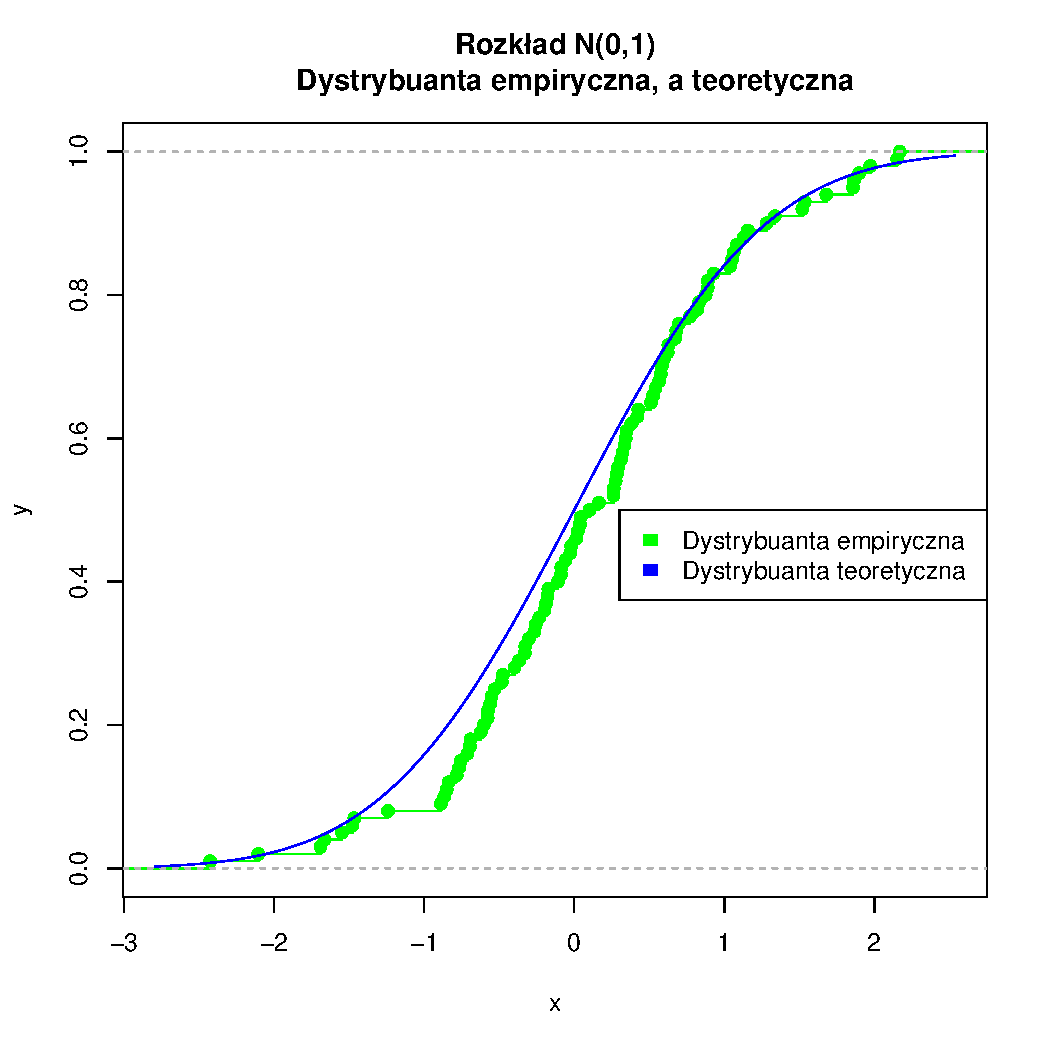
\includegraphics[width=\maxwidth]{figure/unnamed-chunk-1-1} 

}




{\centering 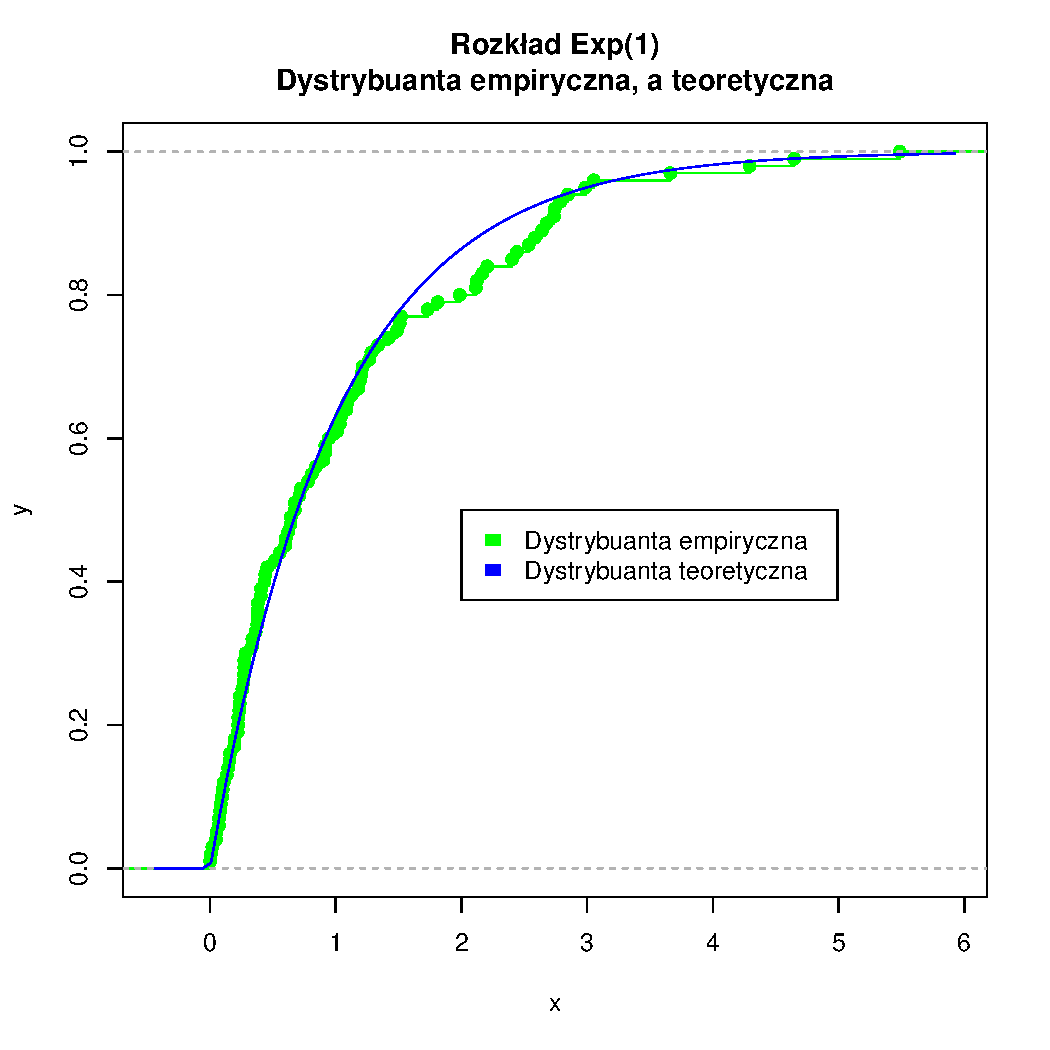
\includegraphics[width=\maxwidth]{figure/unnamed-chunk-1-2} 

}


\end{knitrout}
\newpage
\section{Zadanie 2.}
\begin{knitrout}
\definecolor{shadecolor}{rgb}{0.969, 0.969, 0.969}\color{fgcolor}\begin{kframe}
\begin{alltt}
\hlstd{Symulator} \hlkwb{<-} \hlkwa{function}\hlstd{(}\hlkwc{F}\hlstd{,} \hlkwc{M}\hlstd{=}\hlnum{1000}\hlstd{,} \hlkwc{alpha}\hlstd{=}\hlnum{0.05}\hlstd{,} \hlkwc{n}\hlstd{=}\hlnum{100}\hlstd{,} \hlkwc{R}\hlstd{)\{}
  \hlstd{eps} \hlkwb{<-} \hlstd{(}\hlkwd{log}\hlstd{(}\hlnum{2}\hlopt{/}\hlstd{alpha)}\hlopt{/}\hlstd{(}\hlnum{2}\hlopt{*}\hlstd{n))}\hlopt{^}\hlstd{(}\hlnum{1}\hlopt{/}\hlnum{2}\hlstd{)}
  \hlstd{L} \hlkwb{<-} \hlkwa{function}\hlstd{(}\hlkwc{x}\hlstd{,} \hlkwc{E}\hlstd{)\{}
    \hlkwd{max}\hlstd{(}\hlkwd{E}\hlstd{(x)} \hlopt{-} \hlstd{eps,} \hlnum{0}\hlstd{)\}}
  \hlstd{U} \hlkwb{<-} \hlkwa{function}\hlstd{(}\hlkwc{x}\hlstd{,} \hlkwc{E}\hlstd{)\{}
    \hlkwd{min}\hlstd{(}\hlkwd{E}\hlstd{(x)} \hlopt{+} \hlstd{eps,} \hlnum{1}\hlstd{)\}}
  \hlstd{I} \hlkwb{<-} \hlnum{0}
  \hlkwa{for} \hlstd{(b} \hlkwa{in} \hlnum{1}\hlopt{:}\hlstd{M)\{}
    \hlstd{X} \hlkwb{<-} \hlkwd{R}\hlstd{(n)}
    \hlstd{G} \hlkwb{<-} \hlkwd{c}\hlstd{(}\hlnum{1}\hlopt{:}\hlnum{100}\hlstd{)}
    \hlstd{D} \hlkwb{<-} \hlkwd{c}\hlstd{(}\hlnum{1}\hlopt{:}\hlnum{100}\hlstd{)}
    \hlstd{E} \hlkwb{<-} \hlkwd{ecdf}\hlstd{(X)}
    \hlstd{x} \hlkwb{<-} \hlkwd{seq}\hlstd{(}\hlopt{-}\hlnum{5}\hlstd{,} \hlnum{5}\hlstd{,} \hlkwc{length}\hlstd{=}\hlnum{100}\hlstd{)}
    \hlstd{l} \hlkwb{<-} \hlnum{0}
    \hlkwa{for} \hlstd{(i} \hlkwa{in} \hlnum{1}\hlopt{:}\hlnum{100}\hlstd{)\{}
      \hlkwa{if} \hlstd{(}\hlkwd{L}\hlstd{(x[i], E)}\hlopt{<=}\hlkwd{F}\hlstd{(x[i])} \hlopt{&} \hlkwd{F}\hlstd{(x[i])} \hlopt{<=} \hlkwd{U}\hlstd{(x[i], E))\{}
        \hlstd{l} \hlkwb{<-} \hlstd{l} \hlopt{+}\hlnum{1}\hlstd{\}}
    \hlstd{\}}
    \hlkwa{if}\hlstd{(l}\hlopt{==}\hlnum{100}\hlstd{)\{}
      \hlstd{I} \hlkwb{<-} \hlstd{I} \hlopt{+}\hlnum{1}\hlstd{\}}
    \hlstd{\}}
  \hlkwd{return}\hlstd{(I)}
\hlstd{\}}
\end{alltt}
\end{kframe}
\end{knitrout}

Procent przypadków, w których wykres dystyrbuanty $F$ leży pomiędzy wykresami funkcji $L$ i $U$ dla $F = \Phi$
\begin{knitrout}
\definecolor{shadecolor}{rgb}{0.969, 0.969, 0.969}\color{fgcolor}\begin{kframe}
\begin{alltt}
\hlkwd{Symulator}\hlstd{(pnorm,} \hlkwc{R}\hlstd{=rnorm)}\hlopt{/}\hlnum{10}
\end{alltt}
\begin{verbatim}
## [1] 96.9
\end{verbatim}
\end{kframe}
\end{knitrout}

Procent przypadków, w których wykres dystyrbuanty $F$ leży pomiędzy wykresami funkcji $L$ i $U$ dla $F$ = dystrybuanta rozkładu wykładniczego z parametrem $\lambda = 1$
\begin{knitrout}
\definecolor{shadecolor}{rgb}{0.969, 0.969, 0.969}\color{fgcolor}\begin{kframe}
\begin{alltt}
\hlkwd{Symulator}\hlstd{(pexp,} \hlkwc{R}\hlstd{=rexp)}\hlopt{/}\hlnum{10}
\end{alltt}
\begin{verbatim}
## [1] 97.7
\end{verbatim}
\end{kframe}
\end{knitrout}
\newpage
\section{Zadanie 3.}
\begin{knitrout}
\definecolor{shadecolor}{rgb}{0.969, 0.969, 0.969}\color{fgcolor}

{\centering 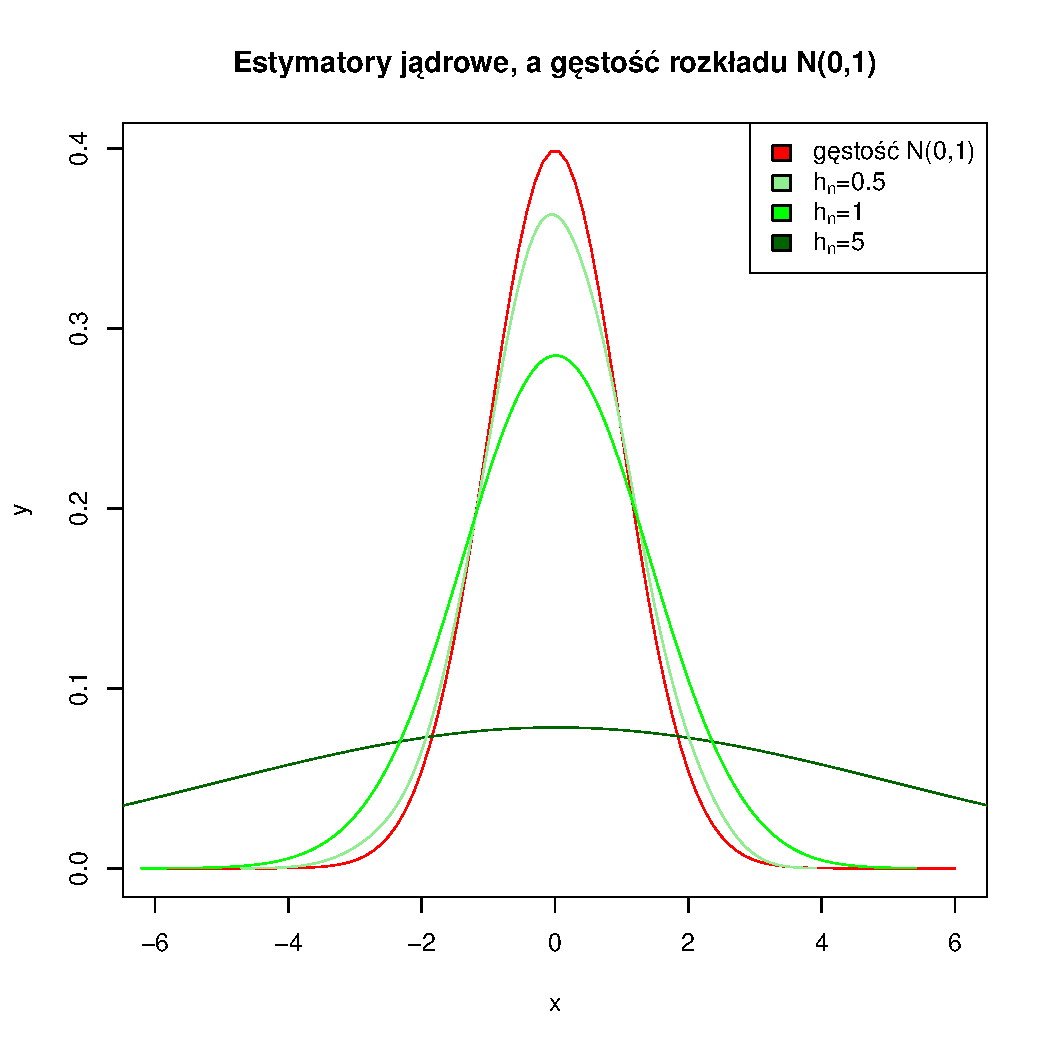
\includegraphics[width=\maxwidth]{figure/unnamed-chunk-5-1} 

}


\end{knitrout}

\textbf{Obserwacja:}
Im szerokość pasma większa, tym wykres gładszy.
\begin{knitrout}
\definecolor{shadecolor}{rgb}{0.969, 0.969, 0.969}\color{fgcolor}

{\centering 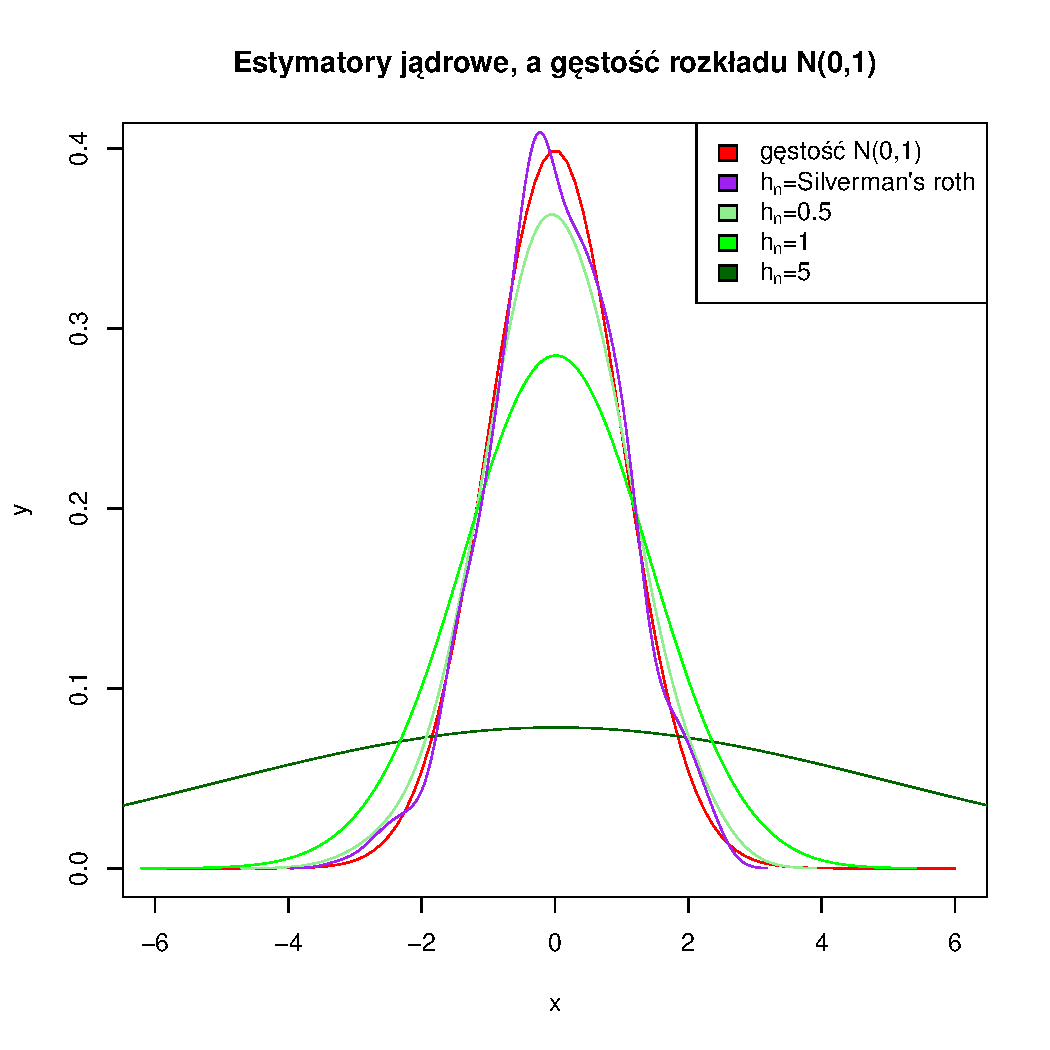
\includegraphics[width=\maxwidth]{figure/unnamed-chunk-6-1} 

}


\end{knitrout}

\newpage
\section{Zadanie 4.}
\begin{knitrout}
\definecolor{shadecolor}{rgb}{0.969, 0.969, 0.969}\color{fgcolor}

{\centering 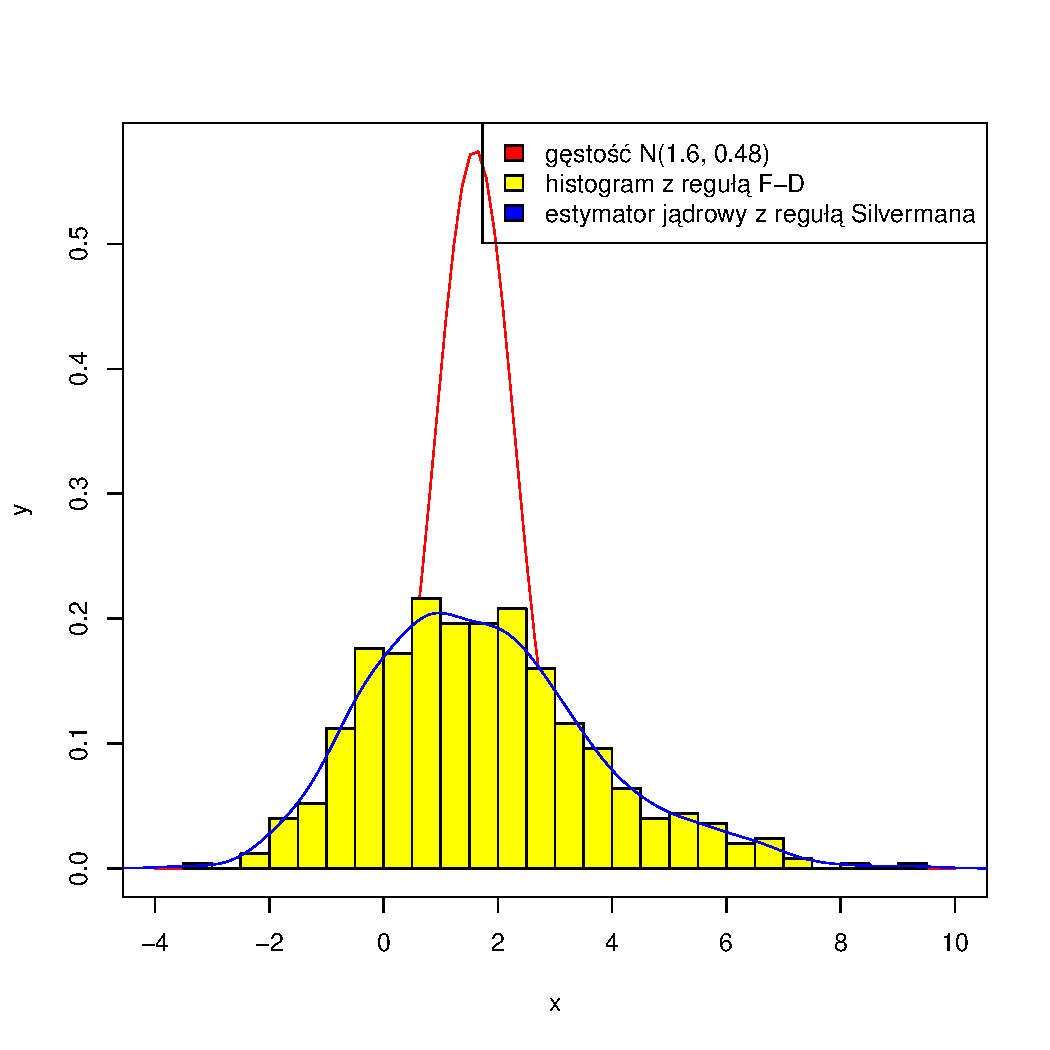
\includegraphics[width=\maxwidth]{figure/unnamed-chunk-7-1} 

}


\end{knitrout}

Estymator jądrowy wydaje się lepszy.
\end{document}
